\chapter{需求分析}
本项目的需求分析方面很简单,也很明确。这里选用数据流图(DFD)来表达。
\begin{center}
  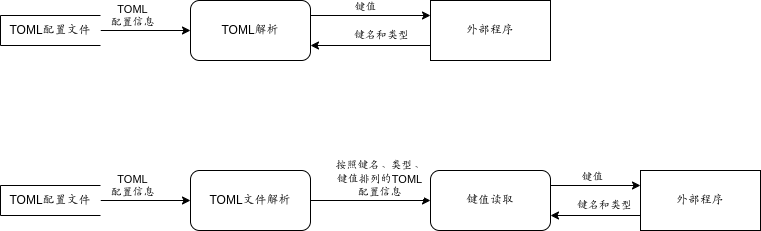
\includegraphics[width=\textwidth]{images/数据流图.png}
\end{center}

此图由draw.io绘图工具绘制后导出。


\chapter{设计}


\section{流程图}
本项目规模很小,并且使用的编程语言是面向结构的C语言,所以使用流程图来设计。

下面的流程图是针对本项目中的示例程序,在实际使用中,读取文件方面的操作由相关调用代码自行处理。
\begin{center}
  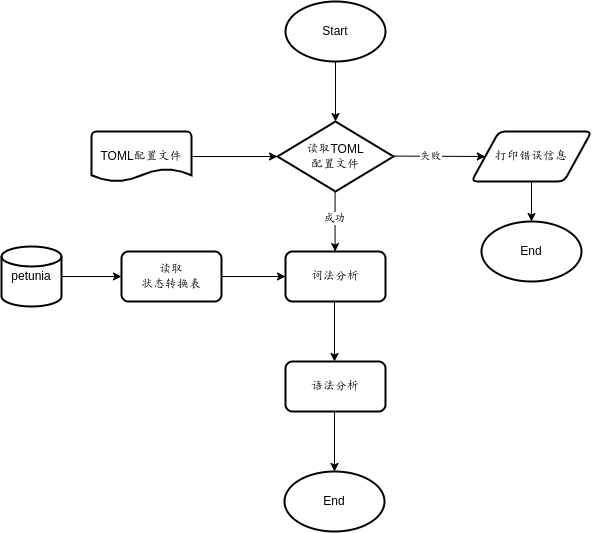
\includegraphics[width=0.8\textwidth]{images/流程图.png}
\end{center}


\section{词法分析}


\subsection{状态转换图}


\subsubsection{注释(comment)}
\noindent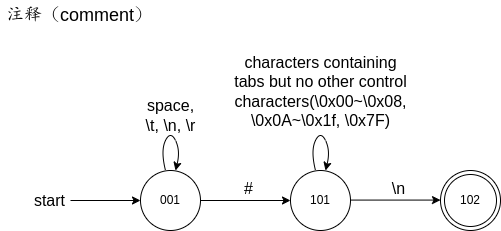
\includegraphics[width=0.6\textwidth]{images/状态转换图之注释.png}


\subsubsection{非数字开头祼键}
\noindent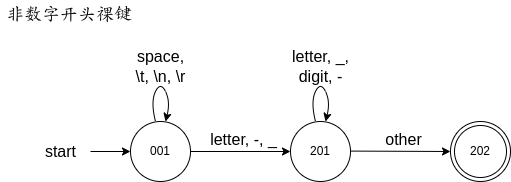
\includegraphics[width=0.6\textwidth]{images/状态转换图之非数字祼键.png}


\subsubsection{运算符}
\noindent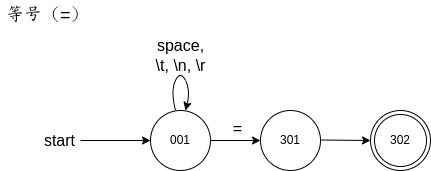
\includegraphics[width=0.5\textwidth]{images/状态转换图之等号.png}


\subsubsection{界符}
\noindent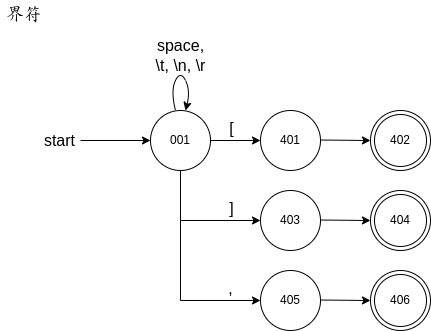
\includegraphics[width=0.6\textwidth]{images/状态转换图之界符.png}


\subsubsection{字符串(string)}
\noindent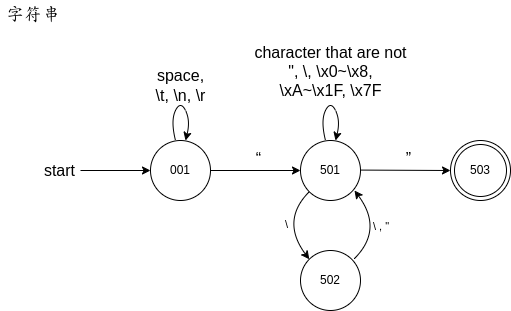
\includegraphics[width=0.6\textwidth]{images/状态转换图之字符串.png}

按照当前的实际需要,暂时不支持多行字符串,另外转义字符目前也只支持反斜杠和双引号。


\subsubsection{整数与浮点数(integer and fractional)}
\noindent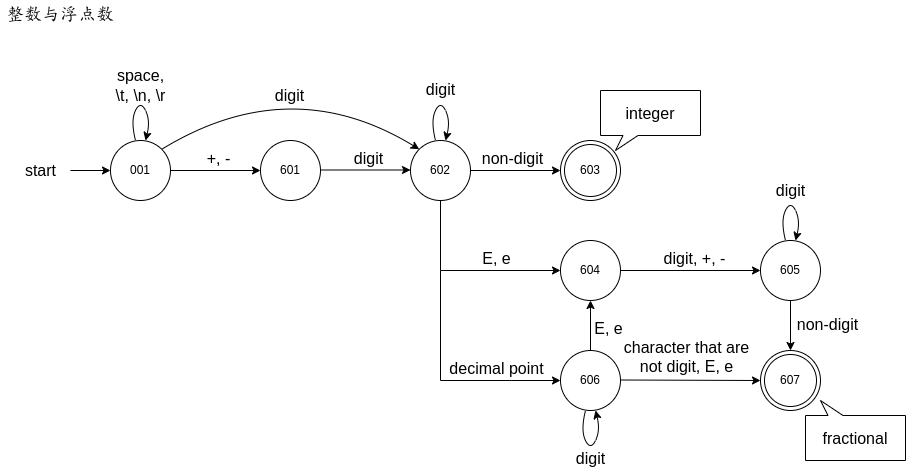
\includegraphics[width=\textwidth]{images/状态转换图之整数与浮点数.png}

目前暂时不支持16进制、8进制。

